\documentclass[conference]{IEEEtran}

\usepackage{graphicx}
\usepackage{booktabs}
\usepackage{amsmath}

\graphicspath{{../images/}}
% The report uses IEEE conference formatting to maintain a
% consistent academic structure for the project update.
% Graphicx is required for displaying generated terrain and
% experiment figures, while booktabs and amsmath support the
% tables and mathematical formulation used in the report.
\begin{document}
% Update 1 report revision
\title{Autonomous Volcanic Terrain Exploration Using a Markov Decision Process\\
{\Large Project Update Report (Update 1)}}
% Team members and course information
\author{
  \IEEEauthorblockN{Shakil Ahmed (2221452042), Fahim Foysal (2233594642),\\
  Shefa Tabassum (2232993042), and Tanvir Ahmed (2231047642)}
  \IEEEauthorblockA{Group 5, CSE 440, Artificial Intelligence, Section 1\\
  North South University \quad$\cdot$\quad Instructor: Dr.\ Mohammad Shifat-E-Rabbi}
}
% The title identifies the central problem addressed by the project,
% while the author block records the complete project team and
% course information for the Update-1 submission.
\maketitle
% The abstract summarizes the project status at the midpoint of
% development. It focuses on the components that were completed
% and integrated at this stage rather than presenting the final
% system as already complete.
\begin{abstract}
This update reports the state of our semester project at the midpoint. The project models autonomous exploration of hazardous volcanic terrain as a Markov Decision Process (MDP). As of this update, all four members' Update-1 work is merged: a seeded procedural terrain generator, the complete MDP formulation with value iteration and policy extraction, a policy-following explorer agent with a simulation loop, matplotlib terrain visualization, and a three-agent baseline experiment framework with CSV and plot outputs. We summarize the design, show preliminary results, and state the plan to the final submission.
\end{abstract}
% This section introduces the environment and explains why an MDP
% is appropriate for the exploration problem. The mathematical
% formulation provides the foundation for the implementation
% components described in the progress section below.
\section{Problem and Approach}

Volcanic environments are dangerous and uncertain: lava flows, craters, gas emissions, and impassable rock threaten any explorer, and a rover's movements on loose terrain are unreliable. Our project asks an autonomous agent, starting from a base station on a grid map, to collect science samples while avoiding hazards and surviving.

Because the task is sequential decision-making under uncertainty, we model it as an MDP $(\mathcal{S}, \mathcal{A}, P, R, \gamma)$ and solve it exactly with value iteration:
% The Bellman update is included to connect the theoretical MDP
% formulation directly to the value-iteration implementation.
% Each action is evaluated using both its immediate reward and
% the discounted value of possible future states.
\begin{equation}
  V(s) \leftarrow \max_{a} \sum_{s'} P(s' \mid s, a)\left[ R(s, a, s') + \gamma V(s') \right].
\end{equation}
States are walkable grid cells; actions are the four movement directions plus \textsc{stay} and \textsc{scan}; movement succeeds as intended with probability $0.75$, drifts sideways with probability $0.10$ each, and stalls with probability $0.05$; rewards range from $+20$ (science) to $-100$ (lava, fatal); and $\gamma = 0.90$.
% Summary of contributions completed by each group member
\section{Progress by Member}
% Terrain generation and MDP implementation
% The progress section records the implementation completed by
% each group member at the midpoint of the project.
% The responsibilities are separated by system component so
% that individual contributions can be identified clearly.
\subsubsection{Member 1: terrain and MDP core} Repository structure and configuration system; a seeded procedural terrain generator over seven cell types with hazard density capped at $0.30$ and CSV save/load; the full MDP formulation; value iteration and optimal policy extraction.

\subsubsection{Member 2: agent and simulation} An \texttt{MDPExplorerAgent} that starts at the base station, queries the policy, and samples real outcomes from the transition model; tracking of reward, hazards entered, science collected, and survival; a simulation loop with a step budget and coverage target and a mission summary.
% Explorer agent and simulation framework
\subsubsection{Member 3: visualization} Matplotlib rendering of the terrain grid with a distinct color per cell type, title, and legend (Fig.~\ref{fig:terrain}); example maps generated across several seeds; a layout-test exploration map (clearly labeled as a sample path, to be replaced by the real agent path).
% The performance plot provides a visual summary of the first
% experimental comparison between the three decision strategies.
% Plotting the metrics together makes differences between the
% MDP, greedy, and random agents easier to identify than inspecting
% the raw numerical output alone.
\subsubsection{Member 4: experiments} A comparison harness running three agents on identical terrains: the MDP agent, a greedy nearest-unvisited baseline, and a random-walk baseline; shared metrics (reward, coverage, hazards, science, survival, steps); automatic CSV and performance-plot generation (Fig.~\ref{fig:performance}).

\begin{figure}[t]
  \centering
  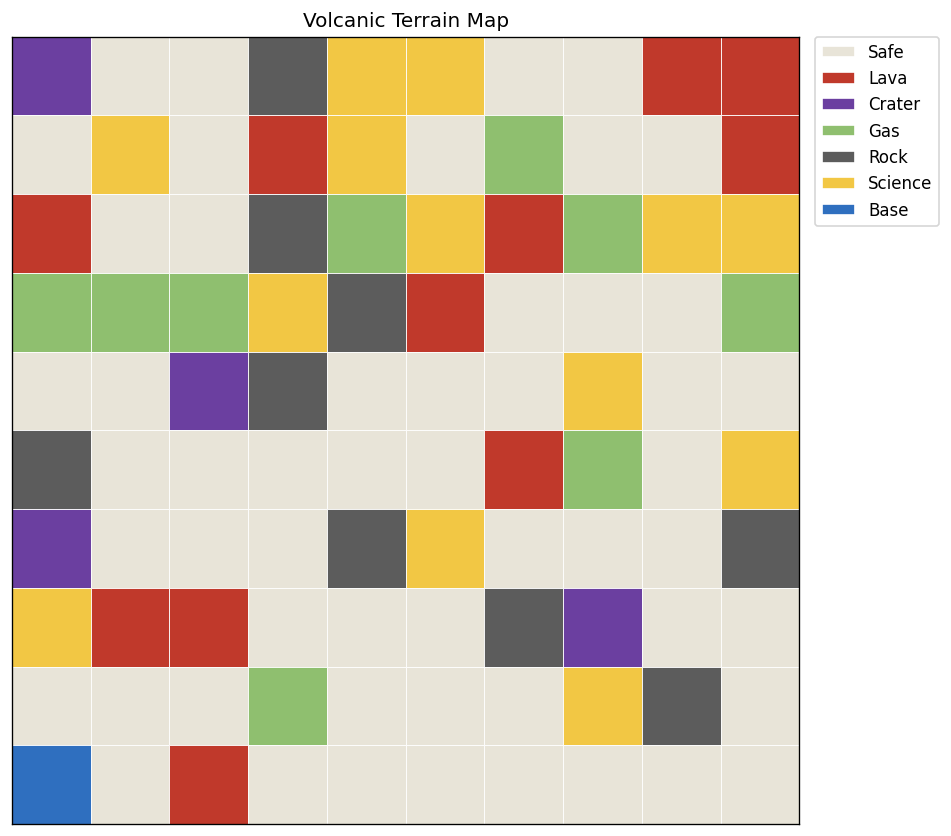
\includegraphics[width=0.31\columnwidth]{terrain_map_seed_1.png}\hfill
  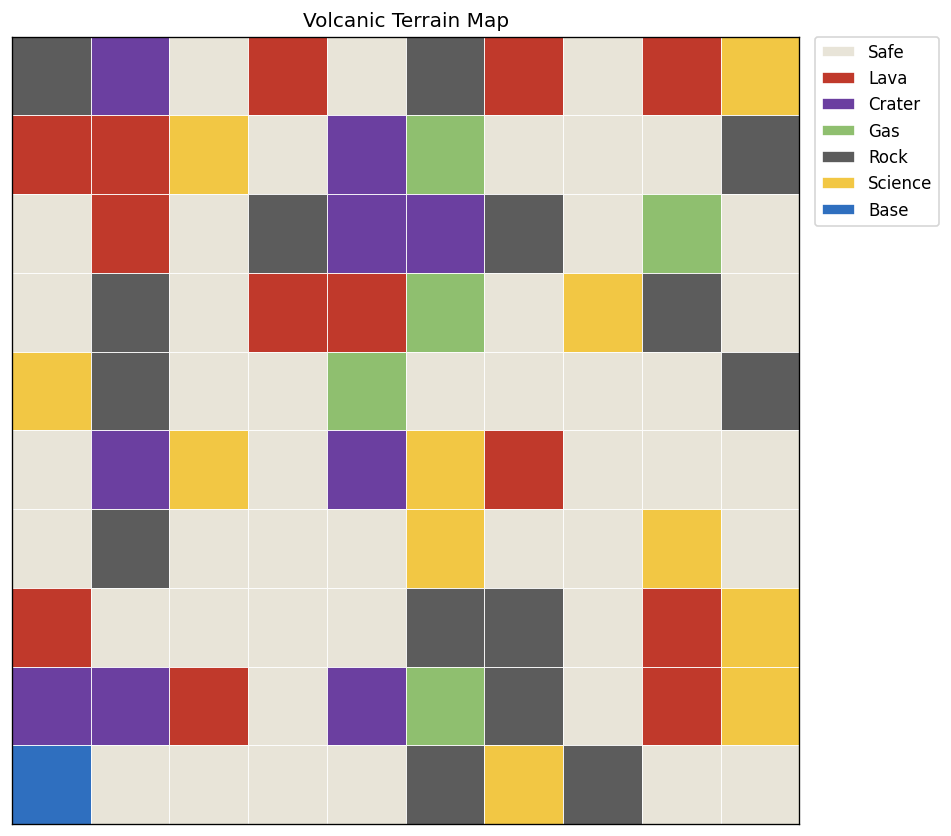
\includegraphics[width=0.31\columnwidth]{terrain_map_seed_7.png}\hfill
  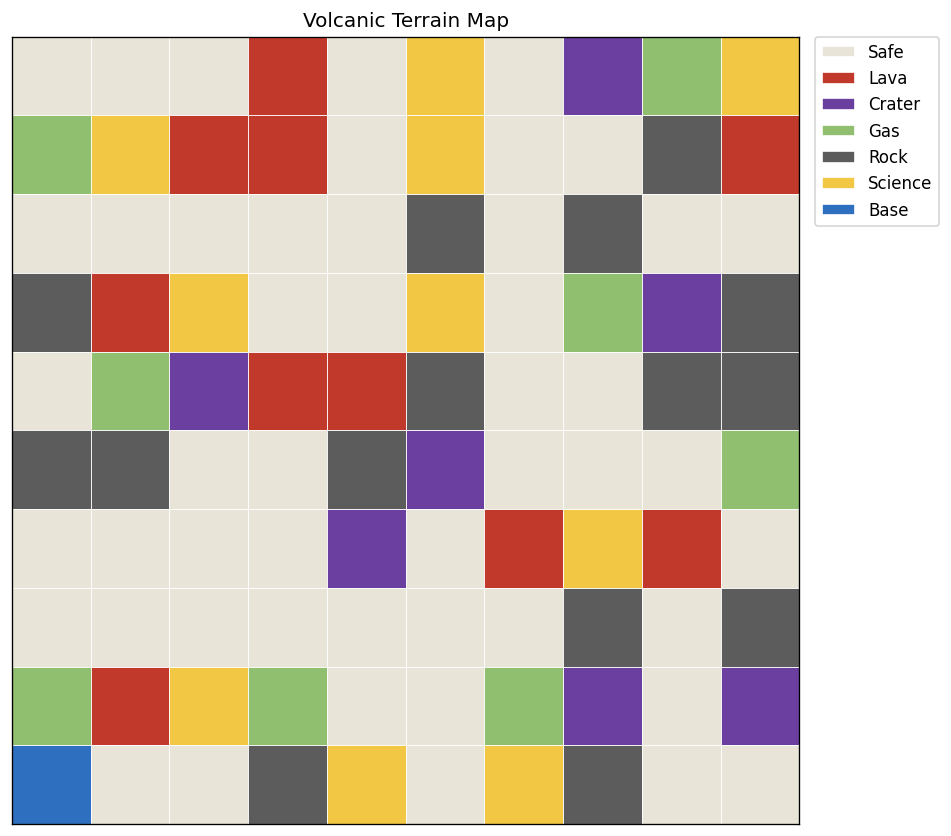
\includegraphics[width=0.31\columnwidth]{terrain_map_seed_23.png}
  \caption{Generated volcanic terrains (seeds 1, 7, 23).}
  \label{fig:terrain}
\end{figure}

\begin{figure}[t]
  \centering
  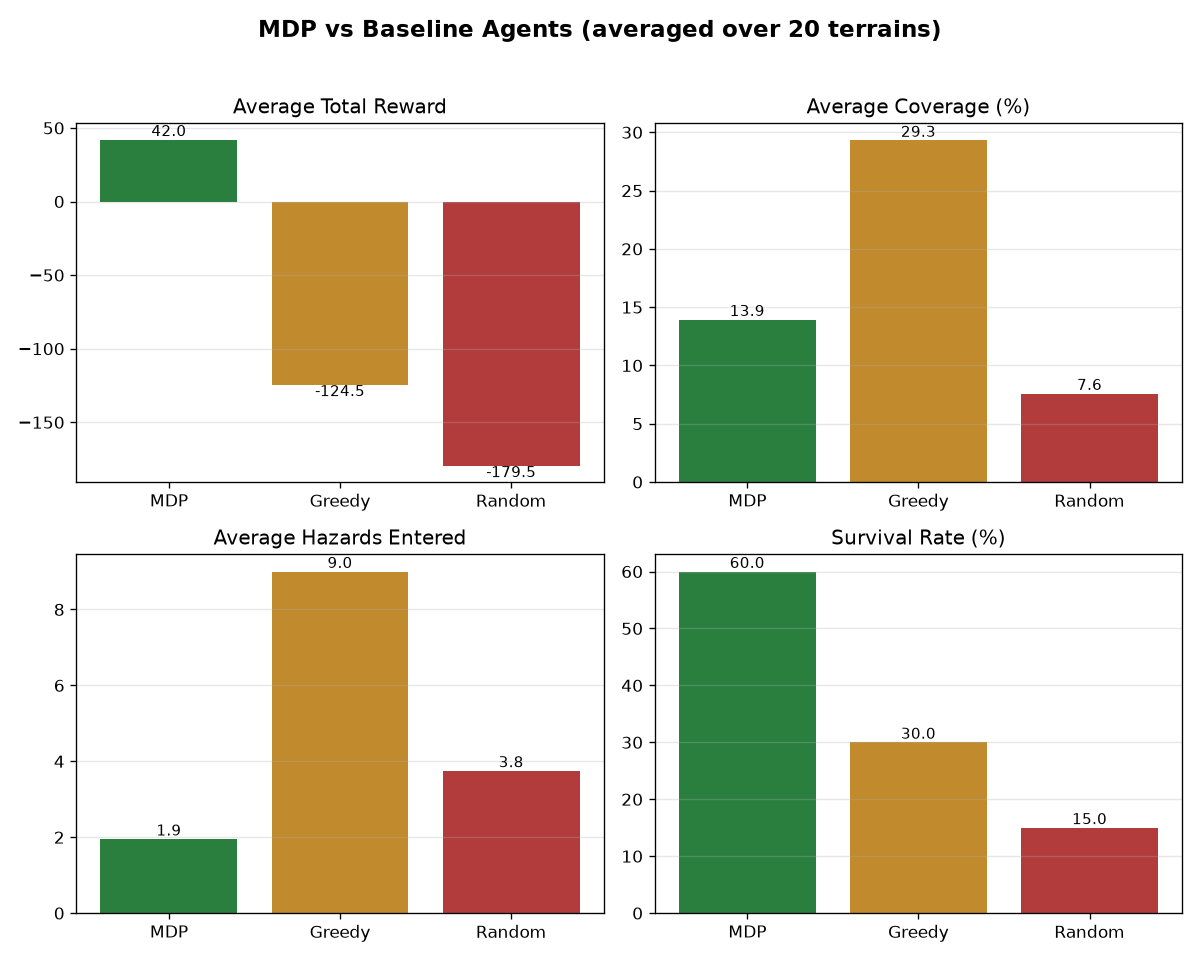
\includegraphics[width=0.95\columnwidth]{performance_plot.png}
  \caption{Preliminary baseline comparison from the experiment framework.}
  \label{fig:performance}
\end{figure}

\section{Preliminary Observations}

The value-iteration policy already routes visibly around lava and craters and toward science points, and the MDP agent outperforms both baselines on reward and survival in the preliminary runs. One issue is identified and scheduled for the next phase: because a science cell pays its reward on every entry, the optimal policy can ``camp'' on a single science cell; we will fix this with a collect-once rule and on-line re-planning.
% The repository statement documents the intended reproducibility
% and collaboration workflow. Per-member branches allow individual
% components to be developed separately, while reviewed pull
% requests provide an explicit integration point before changes
% enter the shared project branch.
\section{Plan to the Final Submission}

\begin{enumerate}
  \item Move the collect-once science rule with re-planning into the core agent (fixing the camping behavior everywhere).
  \item Dynamic hazards: drifting gas clouds and spreading, cooling lava flows, with the agent re-planning after every terrain change.
  \item Render the real simulated agent path on the mission map, replacing the sample path.
  \item Upgrade \texttt{main.py} to run the full pipeline end to end.
  \item Final report (IEEE format), presentation, and the one-minute demo video.
\end{enumerate}

All code is on the group's public GitHub repository, developed through per-member branches and reviewed pull requests, following the mandated layout (\texttt{main.py}, \texttt{README.md}, \texttt{requirements.txt}, \texttt{data/}, \texttt{support/}, \texttt{others/}).

\end{document}
